\chap{Bersyukurlah}

\begin{wrapfigure}{l}{1cm}
\centering
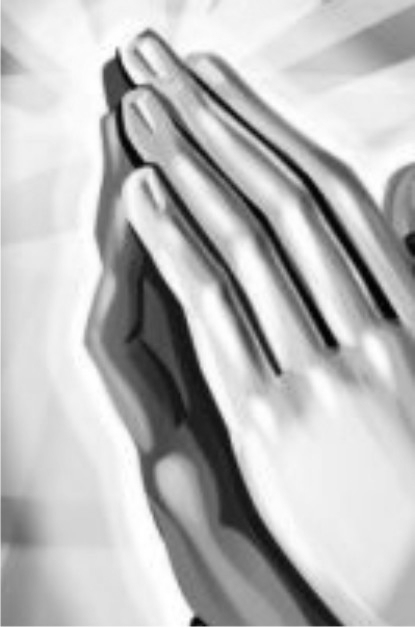
\includegraphics[scale=0.15]{gambar/bersyukur1.png}

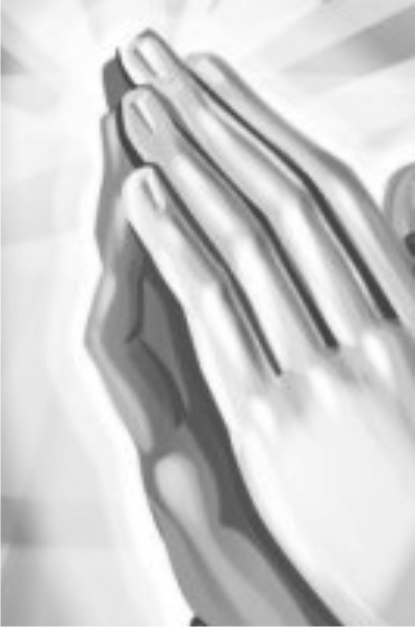
\includegraphics[scale=0.15]{gambar/bersyukur2.png}


\includegraphics[scale=0.15]{gambar/bersyukur3.png}


\includegraphics[scale=0.15]{gambar/bersyukur4.png}

\end{wrapfigure}

{~}

\begin{itemize}[label=\ding{62}]
\item Bersyukurlah bahwa kamu belum siap memiliki segala sesuatu yang kamu inginkan. Seandainya sudah, apalagi yang harus diinginkan?


\item Bersyukurlah apabila kamu tidak tahu sesuatu. Karena itu memberimu kesempatan untuk belajar.

\item Bersyukurlah untuk masa-masa sulit. Di masa itulah kamu tumbuh...

\item Bersyukurlah untuk keterbatasanmu. Karena itu memberimu kesempatan untuk berkembang.
\end{itemize}

\begin{itemize}[label=\ding{62}]
\item Bersyukurlah untuk setiap tantangan baru. Karena itu akan membangun kekuatan dan karaktermu.

\item Bersyukurlah untuk kesalahan yang kamu buat. Itu akan mengajarkan pelajaran yang berharga.

\item Bersyukurlah bila kamu lelah dan letih. Karena itu kamu telah membuat suatu perbedaan.

\item Mungkin mudah untuk kita bersyukur akan hal-hal baik...

\item Hidup yang berkelimpahan datang pada mereka yang juga bersyukur akan masa surut...

\item Rasa syukur dapat mengubah hal yang negatif menjadi positif ...

\item Temukan cara bersyukur akan masalah-masalahmu dan semua itu akan menjadi berkah bagimu ...
\end{itemize}

\sumber{Rahardi, Rian. ``Bersyukurlah.''\\  
www.renungan-harian-kita.blogspot.com.}
